	\newpage
\section{Podręcznik użytkownika}  %6
%Opis jak używać programu. Mogą być z zrzut ekranu razem z opisem.
\hspace{1cm} \textbf{Ekran logowania}

\begin{figure}[!htb]
	\begin{center}
		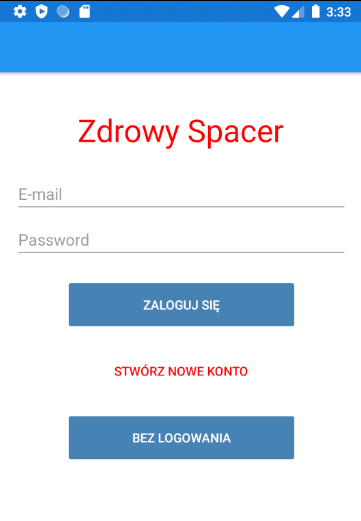
\includegraphics[width=5cm]{rys/login.png}
		\caption{Strona startowa}
		\label{rys:rysunek041}
	\end{center}
\end{figure}
 
Po włączeniu aplikacji widoczna jest strona logowania, którą widać na rysunku 6.1. Jeżeli użytkownik ma już utworzone konto może się zalogować poprzez wprowadzenie swojego adresu email i hasła a nastepnie naciśnięcie przycisku \textbf{zaloguj się}. Jeśli użytkownik chce utworzyć nowe konto to należy wybrać przycisk \textbf{stwórz nowe konto}. \newline

\begin{figure}[!htb]
	\begin{center}
		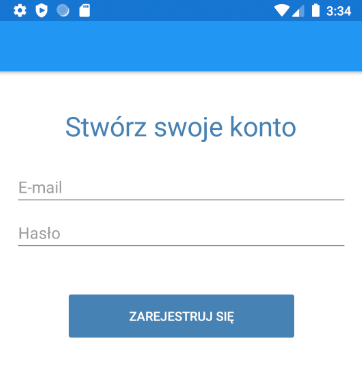
\includegraphics[width=6cm]{rys/register.png}
		\caption{Strona rejestracji}
		\label{rys:rysunek042}
	\end{center}
\end{figure}

Po wybraniu opcji \textbf{stwórz nowe konto} użytkownik zostanie przeniesiony na stronę rejestracji, która jest przedstawiona na rysunku 6.2.
Aby utworzyć nowe konto użytkownik musi wprowadzić prawidłowy adres email oraz hasło o długości minimum 6 znaków a następnie nacisnąć przycisk \textbf{zarejestruj się}. W przypadku poprawnego utworzenia konta użytkownik zostanie przeniesiony na stronę logowania. Jeżeli tworzenie konta się nie powiedzie pojawi się komunikat o błędzie. 


\begin{figure}[!htb]
	\begin{center}
		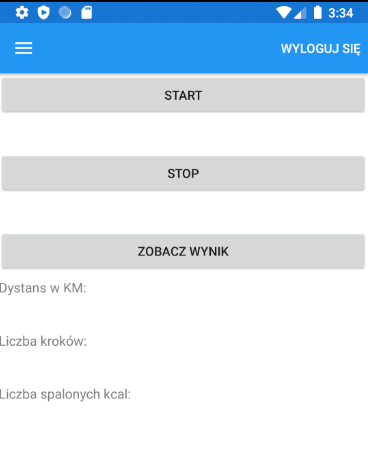
\includegraphics[width=4cm]{rys/glowna_empty.png}
		\caption{Strona główna}
		\label{rys:rysunek043}
	\end{center}
\end{figure}

Na rysunku 6.3 widzimy stronę główną na którą po zalogowaniu zostanie przeniesiony użytkownik na stronę główną. Wybranie przycisku \textbf{wyloguj się} który znajduje się w prawym górnym rogu spowoduje wylogowanie z aplikacji i powrót na stronę logowania. Wybranie ikony menu, która znajduje się w prawym górnym rogu spowoduje wyświetlenie się menu bocznego. Przycisk \textbf{start} należy klknąć w momencie rozpoczęcia spaceru, spowoduje to wyświetlenie adresu lokalizacji startowej. Przycisk \textbf{stop} należy nacisnąć w momencie zakończenia spaceru, zostanie wtedy wyświetlony adres lokalizacji końcowej. Kliknięcie przycisku \textbf{zobacz wynik} będzie skutkowało wyświetleniem przebytego dystansu podanego w kilometrach, liczby wykonanych kroków oraz liczby spalonych kalorii.

\begin{figure}[!htb]
	\begin{center}
		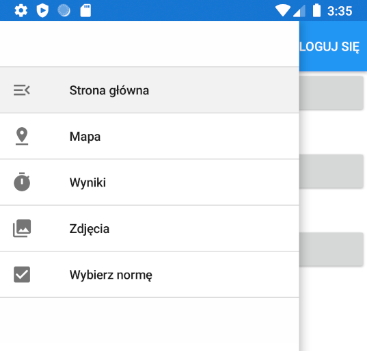
\includegraphics[width=5cm]{rys/menu.png}
		\caption{Widok po włączeniu menu bocznego}
		\label{rys:rysunek044}
	\end{center}
\end{figure}

Na rysunku 6.4 widzimy menu z którego użytkownik ma do wyboru pięć opcji: strona główna, mapa, wyniki, zdjęcia, wybierz normę. W zależności od tego, którą opcję wybierze użytkownik zostanie on przekierowany na odpowiadającą swojemu wyborowi stronę.

\begin{figure}[!htb]
	\begin{center}
		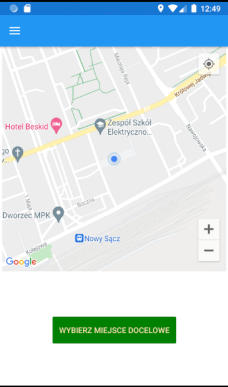
\includegraphics[width=4cm]{rys/ZZp1.png}
		\caption{Mapa}
		\label{rys:rysunek045}
	\end{center}
\end{figure}

Po wybraniu mapy widoczna będzie mapa wraz ze znacznikiem określającym obecną lokalizację użytkownika oraz przycisk \textbf{Wybierz miejsce docelowe} tak jak to jest pokazane na rysunku 6.5.

\begin{figure}[!htb]
	\begin{center}
		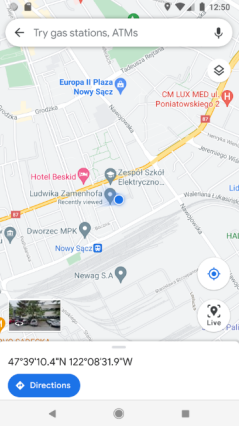
\includegraphics[width=4cm]{rys/ZZp2.png}
		\caption{Google Maps i wybór miejsca docelowego}
		\label{rys:rysunek046}
	\end{center}
\end{figure}

Na rysunku 6.6 widzimy mapę z Google Maps, która otwiera się po kliknięciu przycisku \textbf{Wybierz miejsce docelowe}. Korzystając z niej użytkownik może wpisać adres miejsca docelowego co będzie skutkowało wyznaczeniem przez Google Maps trasy z obecnej lokalizacji do wyznaczonego celu.

\begin{figure}[!htb]
	\begin{center}
		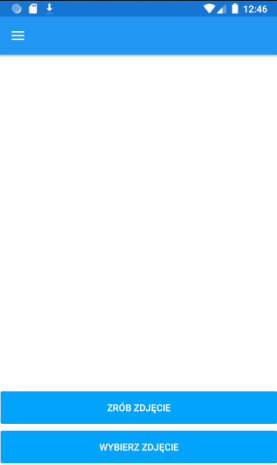
\includegraphics[width=3cm]{rys/ZZf1.png}
		\caption{Zakładka Zdjęcia}
		\label{rys:rysunek047}
	\end{center}
\end{figure}

Po wybraniu z menu bocznego opcji \textbf{zdjęcia} użytkownik zostanie przeniesony na stronę, która jest pokazana na rysunku 6.7. Znajdują się tu dwa przyciski \textbf{zrób zdjęcie} oraz \textbf{wybierz zdjęcie}.

\begin{figure}[!htb]
	\begin{center}
		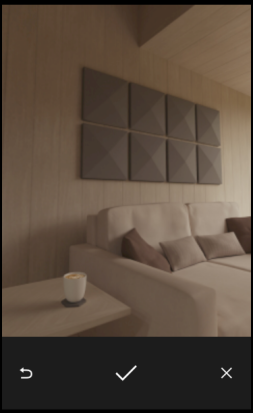
\includegraphics[width=3cm]{rys/ZZf2.png}
		\caption{Aparat}
		\label{rys:rysunek048}
	\end{center}
\end{figure}

Po kliknięciu przycisku \textbf{zrób zdjęcie} otwarty zostanie aparat w telefonie i możliwe będzie wykonanie zdjęcia co zostało pokazane na rysunku 6.8. Wykonane zdjęcie zostanie wyświetlone na stronie w miejscu nad przyciskami.

\begin{figure}[!htb]
	\begin{center}
		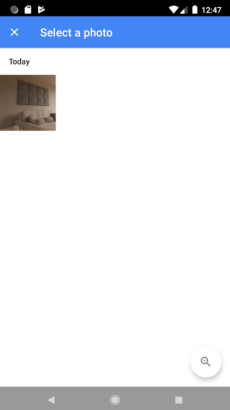
\includegraphics[width=2.5cm]{rys/ZZf3.png}
		\caption{Wybór zdjęcia z galerii}
		\label{rys:rysunek049}
	\end{center}
\end{figure}

Na rysunku 6.9 pokazany jest widok po kliknięciu przycisku \textbf{wybierz zdjęcie}. Otwarta zostaje galeria telefonu i możliwe jest wybranie dowolnego wcześniej wykonanego zdjęcia które następnie zostanie wyświetlone na stronie. 